\input{../utils/preamble}
\createdgmtitle{14}

\usepackage{tikz}

\usetikzlibrary{arrows,shapes,positioning,shadows,trees}
%--------------------------------------------------------------------------------
\begin{document}
%--------------------------------------------------------------------------------
\begin{frame}[noframenumbering,plain]
%\thispagestyle{empty}
\titlepage
\end{frame}
%=======
\begin{frame}{Recap of previous lecture}
		\vspace{-0.3cm}
		\[
		\ba_{\bz}(t) = \frac{\partial L(\by)}{\partial \bz(t)}; \quad \ba_{\btheta}(t) = \frac{\partial L(\by)}{\partial \btheta(t)} \text{-- adjoint functions}.
		\]
		\vspace{-0.3cm}
	\begin{block}{Theorem (Pontryagin)}
	\vspace{-0.6cm}
	\[
		\frac{d \ba_{\bz}(t)}{dt} = - \ba_{\bz}(t)^T \cdot \frac{\partial f(\bz(t), t, \btheta)}{\partial \bz}; \quad \frac{d \ba_{\btheta}(t)}{dt} = - \ba_{\bz}(t)^T \cdot \frac{\partial f(\bz(t), t, \btheta)}{\partial \btheta}.
	\]
	\vspace{-0.6cm}
	\end{block}
	\begin{block}{Forward pass}
		\vspace{-0.5cm}
		\[
		\bz(t_1) = \int^{t_1}_{t_0} f(\bz(t), t, \btheta) d t  + \bz_0 \quad \Rightarrow \quad \text{ODE Solver}
		\]
		\vspace{-0.6cm}
	\end{block}
	\begin{block}{Backward pass}
		\vspace{-0.6cm}
		\begin{equation*}
			\left.
			{\footnotesize 
				\begin{aligned}
					\frac{\partial L}{\partial \btheta(t_0)} &= \ba_{\btheta}(t_0) =  - \int_{t_1}^{t_0} \ba_{\bz}(t)^T \frac{\partial f(\bz(t), t, \btheta)}{\partial \btheta(t)} dt + 0 \\
					\frac{\partial L}{\partial \bz(t_0)} &= \ba_{\bz}(t_0) =  - \int_{t_1}^{t_0} \ba_{\bz}(t)^T \frac{\partial f(\bz(t), t, \btheta)}{\partial \bz(t)} dt + \frac{\partial L}{\partial \bz(t_1)} \\
					\bz(t_0) &= - \int^{t_0}_{t_1} f(\bz(t), t, \btheta) d t  + \bz_1.
				\end{aligned}
			}
			\right\rbrace
			\Rightarrow
			\text{ODE Solver}
		\end{equation*}
		\vspace{-0.4cm} 
	\end{block}
	\myfootnotewithlink{https://arxiv.org/abs/1806.07366}{Chen R. T. Q. et al. Neural Ordinary Differential Equations, 2018}   
\end{frame}
%=======
\begin{frame}{Recap of previous lecture}
	\begin{block}{Continuous-in-time normalizing flows}
		\vspace{-0.5cm}
		\[
			\frac{d\bz(t)}{dt} = f(\bz(t), t, \btheta); \quad \frac{d \log p(\bz(t), t)}{d t} = - \text{tr} \left( \frac{\partial f (\bz(t), t, \btheta)}{\partial \bz(t)} \right).
		\]
		\vspace{-0.7cm}
	\end{block}
	\begin{block}{Theorem (Picard)}
		If $f$ is uniformly Lipschitz continuous in $\bz$ and continuous in $t$, then the ODE has a \textbf{unique} solution.
	\end{block}
	\begin{block}{Forward transform + log-density}
		\vspace{-0.4cm}
		\[
			\begin{bmatrix}
				\bx \\
				\log p(\bx | \btheta)
			\end{bmatrix}
			= 
			\begin{bmatrix}
				\bz \\
				\log p(\bz)
			\end{bmatrix} + 
			\int_{t_0}^{t_1} 
			\begin{bmatrix}
				f(\bz(t), t, \btheta) \\
				- \text{tr} \left( \frac{\partial f(\bz(t), t, \btheta)}{\partial \bz(t)} \right) 
			\end{bmatrix} dt.
		\]
		\vspace{-0.4cm}
	\end{block}	
	\begin{block}{Hutchinson's trace estimator}
		\vspace{-0.3cm}
		\[
		   \log p(\bz(t_1)) = \log p(\bz(t_0)) - \mathbb{E}_{p(\bepsilon)} \int_{t_0}^{t_1} \left[ {\color{violet}\bepsilon^T \frac{\partial f}{\partial \bz}} \bepsilon \right] dt.
		\]
	\end{block}
	\myfootnotewithlink{https://arxiv.org/abs/1810.01367}{Grathwohl W. et al. FFJORD: Free-form Continuous Dynamics for Scalable Reversible Generative Models, 2018} 
\end{frame}
%=======
\begin{frame}{Recap of previous lecture}
	\vspace{-0.2cm}
	\begin{block}{SDE basics}
		Let define stochastic process $\bx(t)$ with initial condition $\bx(0) \sim p_0(\bx)$:
		\[
			d\bx = \mathbf{f}(\bx, t) dt + g(t) d \bw, 
		\]
		where $\bw(t)$ is the standard Wiener process (Brownian motion)
		\vspace{-0.2cm}
		\[		
			\bw(t) - \bw(s) \sim \cN(0, (t - s) \bI), \quad d \bw = \bepsilon \cdot \sqrt{dt}, \, \text{where } \bepsilon \sim \cN(0, \bI).
		\]
	\end{block}
	\vspace{-0.5cm}
	\begin{block}{Langevin dynamics}
		Let $\bx_0$ be a random vector. Then under mild regularity conditions for small enough $\eta$ samples from the following dynamics
		\vspace{-0.2cm}
		\[
			\bx_{t + 1} = \bx_t + \eta \frac{1}{2} \nabla_{\bx_t} \log p(\bx_t | \btheta) + \sqrt{\eta} \cdot \bepsilon, \quad \bepsilon \sim \cN(0, \bI).
		\]
		will comes from $p(\bx | \btheta)$.
	\end{block}
	The density $p(\bx | \btheta)$ is a \textbf{stationary} distribution for the Langevin SDE.
	\myfootnotewithlink{https://www.stats.ox.ac.uk/~teh/research/compstats/WelTeh2011a.pdf}{Welling M. Bayesian Learning via Stochastic Gradient Langevin Dynamics, 2011}
\end{frame}
%=======
\begin{frame}{Stochastic differential equation (SDE)}
	\begin{block}{Statement}
		Let $\bx_0$ be a random vector. Then samples from the following dynamics
		\[
			\bx_{t + 1} = \bx_t + \eta \frac{1}{2} \nabla_{\bx_t} \log p(\bx_t | \btheta) + \sqrt{\eta} \cdot \bepsilon, \quad \bepsilon \sim \cN(0, 1).
		\]
		will come from $p(\bx | \btheta)$ under mild regularity conditions for small enough $\eta$ and large enough $t$.
	\end{block}
	\begin{minipage}{0.6\linewidth}
		The density $p(\bx | \btheta)$ is a \textbf{stationary} distribution for this SDE.
	\end{minipage}%
	\begin{minipage}{0.35\linewidth}
		\vspace{-0.2cm}
		\begin{figure}
			\centering
			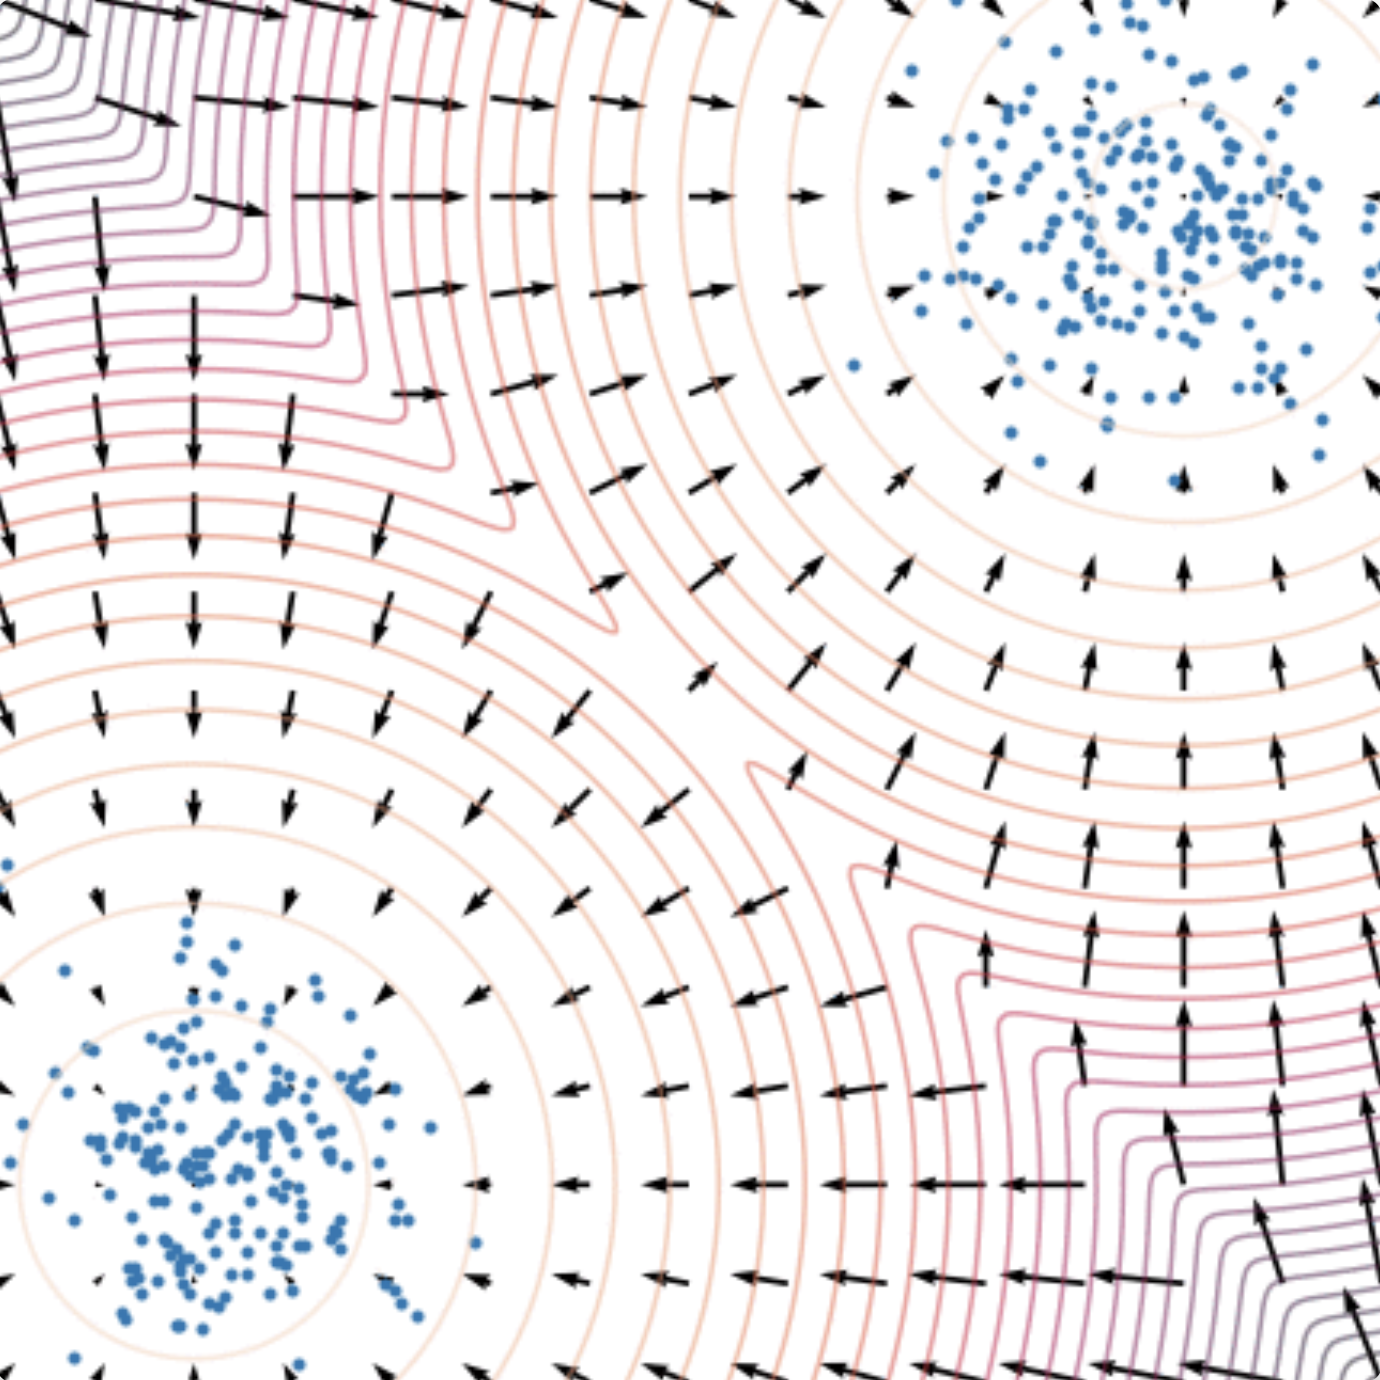
\includegraphics[width=0.9\linewidth]{figs/langevin_dynamic}
		\end{figure}
	\end{minipage}
	\myfootnotewithlink{https://yang-song.github.io/blog/2021/score/}{Song Y. Generative Modeling by Estimating Gradients of the Data Distribution, blog post, 2021} 
	\end{frame}
%=======
\begin{frame}{Outline}
	\tableofcontents
\end{frame}
%=======
\section{Score matching}
%=======
\begin{frame}{Generative models zoo}
	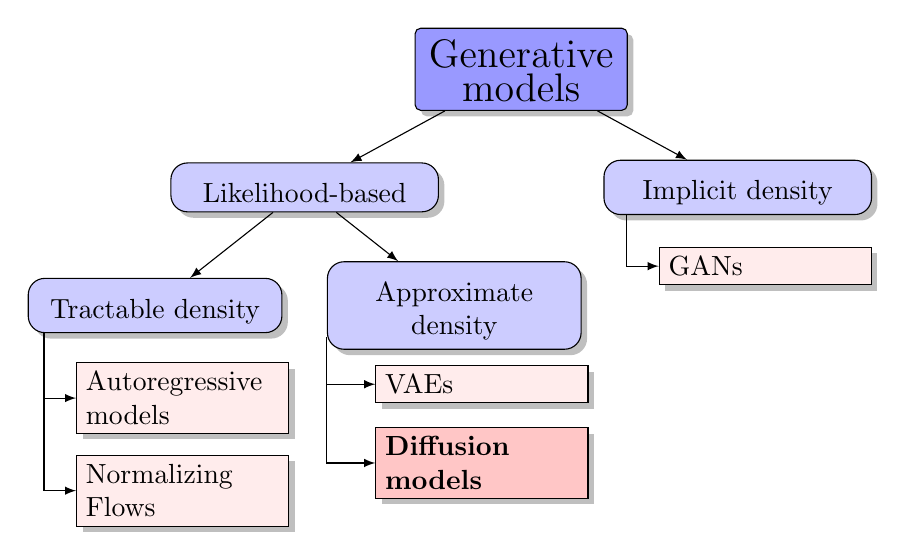
\begin{tikzpicture}[
		basic/.style  = {draw, text width=2cm, drop shadow, rectangle},
		root/.style   = {basic, rounded corners=2pt, thin, text height=1.1em, text width=7em, align=center, fill=blue!40},
		level 1/.style={sibling distance=55mm},
		level 2/.style = {basic, rounded corners=6pt, thin, align=center, fill=blue!20, text height=1.1em, text width=9em, sibling distance=38mm},
		level 3/.style = {basic, rounded corners=6pt, thin,align=center, fill=blue!20, text width=8.5em},
		level 4/.style = {basic, thin, align=left, fill=pink!30, text width=7em},
		level 5/.style = {basic, thin, align=left, fill=pink!90, text width=7em},
		edge from parent/.style={->,draw},
		>=latex]
		
		% root of the the initial tree, level 1
		\node[root] {\Large Generative models}
		% The first level, as children of the initial tree
		child {node[level 2] (c1) {Likelihood-based}
			child {node[level 3] (c11) {Tractable density}}
			child {node[level 3] (c12) {Approximate density}}
		}
		child {node[level 2] (c2) {Implicit density}};
		
		% The second level, relatively positioned nodes
		\begin{scope}[every node/.style={level 4}]
			\node [below of = c11, yshift=-5pt, xshift=10pt] (c111) {Autoregressive models};
			\node [below of = c111, yshift=-5pt] (c112) {Normalizing Flows};
			\node [below of = c12, xshift=10pt] (c121) {VAEs};
			
			\node [below of = c2, xshift=10pt] (c21) {GANs};
		\end{scope}
		
		% The second level, relatively positioned nodes
		\begin{scope}[every node/.style={level 5}]
			\node [below of = c121] (c122) {\textbf{Diffusion \\ models}};
		\end{scope}
		
		% lines from each level 1 node to every one of its "children"
		\foreach \value in {1,2}
		\draw[->] (c11.194) |- (c11\value.west);
		
		\foreach \value in {1,2}
		\draw[->] (c12.194) |- (c12\value.west);
		
		\draw[->] (c2.194) |- (c21.west);
		
	\end{tikzpicture}
\end{frame}
%=======
\begin{frame}{Score matching}
	We could sample from the model using Langevin dynamics if we have $\nabla_{\bx}\log p(\bx| \btheta)$.
	\begin{block}{Fisher divergence}
		\vspace{-0.3cm}
		\[
		D_F(\pi, p) = \frac{1}{2}\bbE_{\pi}\bigl\| \nabla_{\bx}\log p(\bx| \btheta) - \nabla_\bx \log \pi(\bx) \bigr\|^2_2 \rightarrow \min_{\btheta}
		\]
		\vspace{-0.5cm}
	\end{block}
	Let introduce \textbf{score function} $\bs(\bx, \btheta) = \nabla_{\bx}\log p(\bx| \btheta)$. 
	\vspace{-0.2cm}
	\begin{figure}
		\centering
		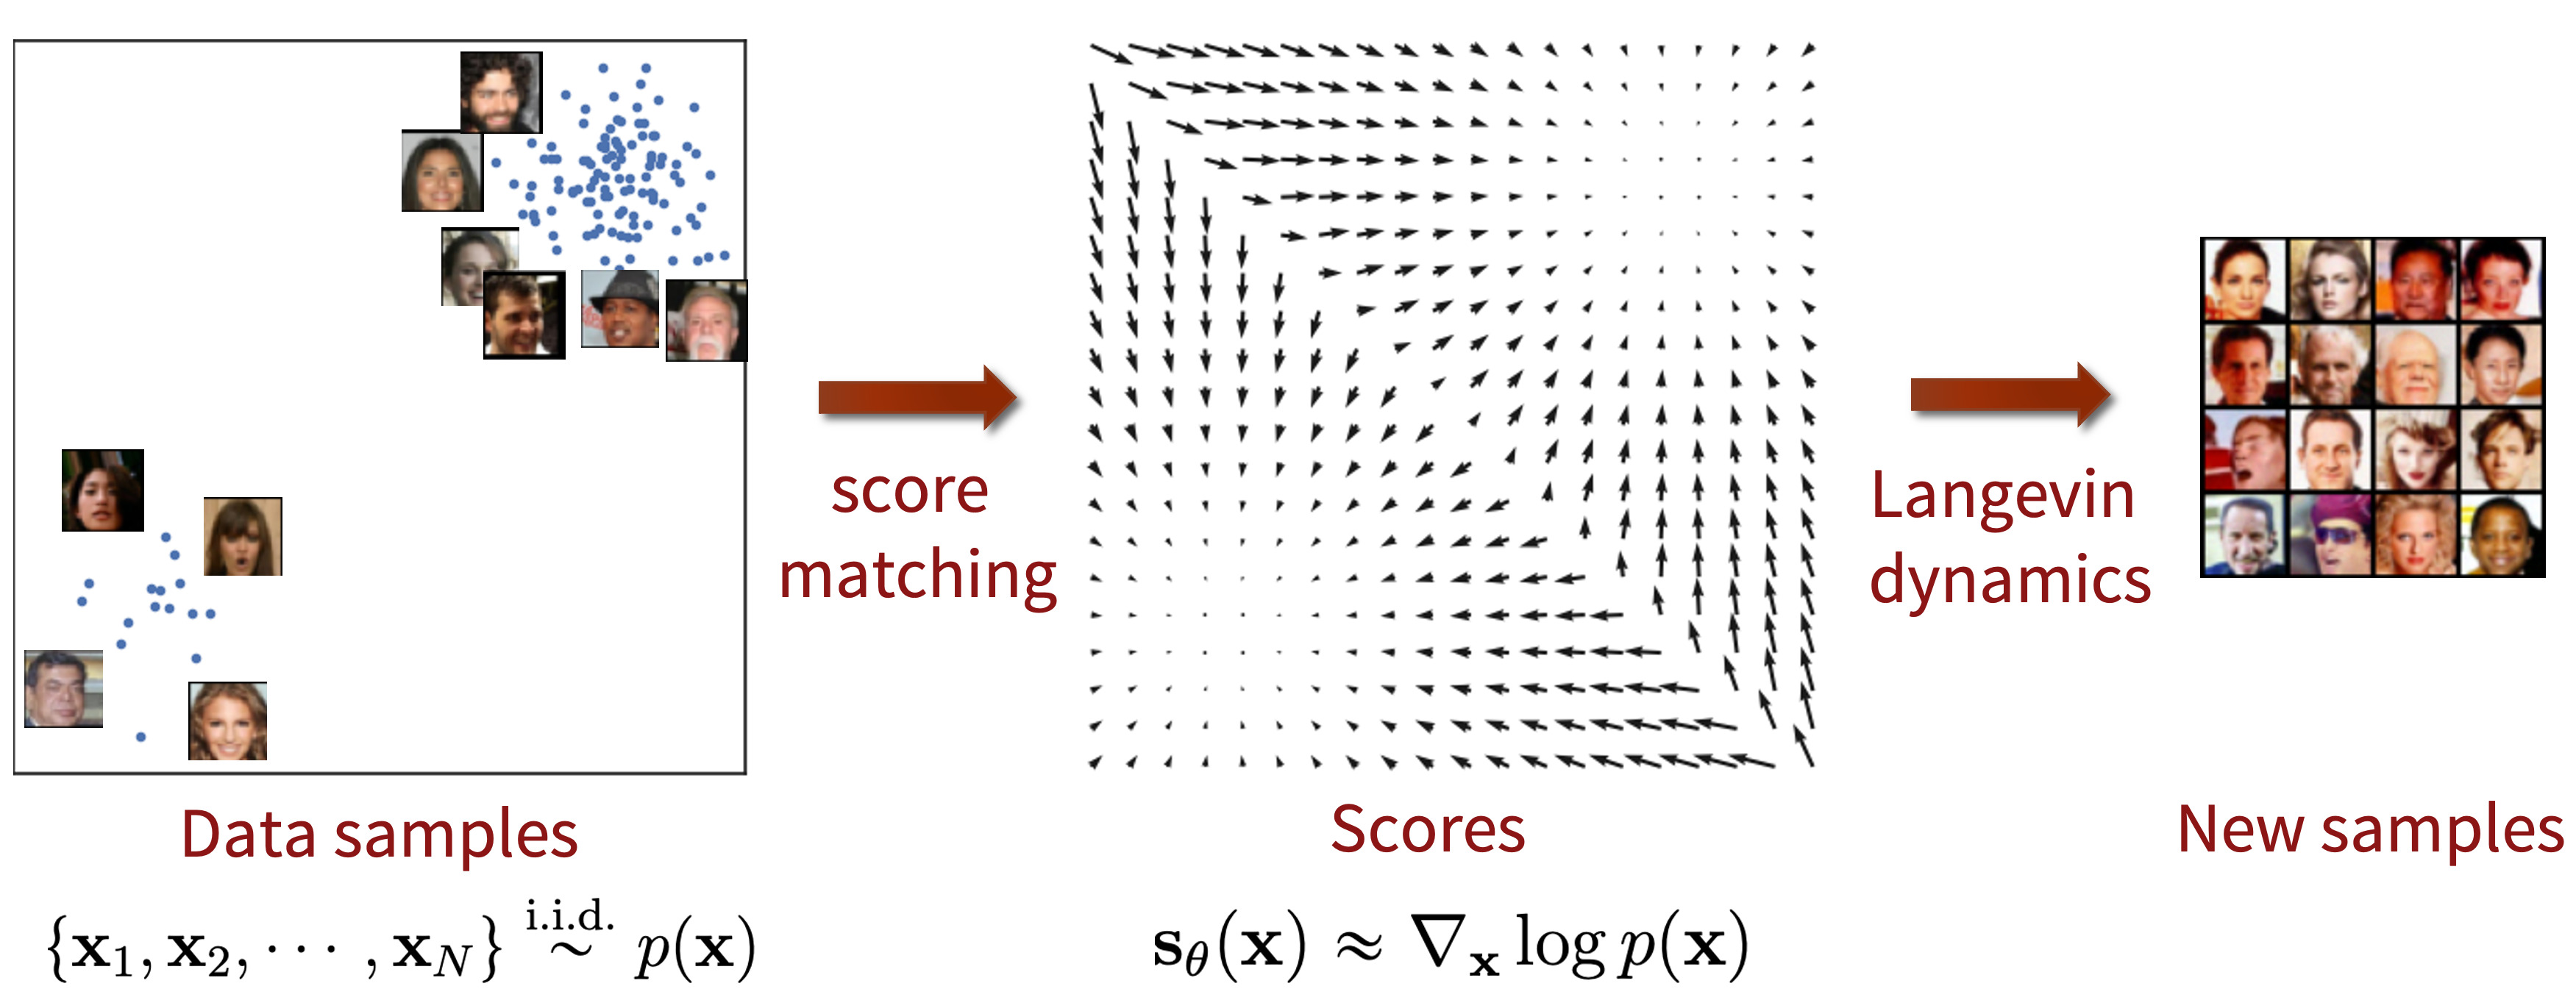
\includegraphics[width=0.75\linewidth]{figs/smld}
	\end{figure}
	\vspace{-0.3cm} 
	\textbf{Problem:} we do not know $\nabla_\bx \log \pi(\bx)$.
	\myfootnotewithlink{https://yang-song.github.io/blog/2021/score/}{Song Y. Generative Modeling by Estimating Gradients of the Data Distribution, blog post, 2021}
\end{frame}
%=======
\begin{frame}{Score matching}
	\begin{block}{Theorem (implicit score matching)}
		Under some regularity conditions, it holds
		\vspace{-0.2cm}
		\[
		\frac{1}{2} \bbE_{\pi}\bigl\| \bs(\bx, \btheta) - \nabla_\bx \log \pi(\bx) \bigr\|^2_2 = \bbE_{\pi}\Bigr[ \frac{1}{2}\| \bs(\bx, \btheta) \|_2^2 + \text{tr}\bigl(\nabla_{\bx} \bs(\bx, \btheta)\bigr) \Bigr] + \text{const}
		\]
		\vspace{-0.6cm}
	\end{block}
	\begin{block}{Proof (only for 1D)}
		\vspace{-0.6cm}
		{\small
			\begin{multline*}
				\bbE_{\pi}\bigl\| s(x) - \nabla_x \log \pi(x) \bigr\|^2_2 = \bbE_{\pi} \bigl[ s(x)^2 + (\nabla_x \log \pi(x))^2 - 2{\color{teal}[s(x) \nabla_x \log \pi(x) ] \bigr] }
			\end{multline*}
			\vspace{-0.8cm}
			\begin{align*}
				{\color{teal}\bbE_{\pi} [{\color{violet}s(x) } \nabla_x \log \pi(x) ] } &= \int {\color{olive}\pi(x) {\color{violet}\nabla_x \log p(x)} \nabla_x \log \pi(x)} d x \\ 
				&= \int {\color{violet}\nabla_x \log p(x) } {\color{olive}\nabla_x \pi(x) } dx = \Bigl.\pi(x) \nabla_x \log p(x) \Bigr|_{-\infty}^{+\infty} \\
				&- \int \nabla^2_x \log p(x)  \pi(x) dx =- \bbE_{\pi} \nabla^2_x \log p(x) =- \bbE_{\pi} \nabla_x s(x)
			\end{align*}
			\[
			\frac{1}{2} \bbE_{\pi}\bigl\| s(x) - \nabla_x \log \pi(x) \bigr\|^2_2 = \bbE_{\pi} \Bigr[\frac{1}{2} s(x)^2 + \nabla_x s(x) \Bigl]+ \text{const}.
			\]
		}
	\end{block}
	\myfootnotewithlink{https://jmlr.org/papers/volume6/hyvarinen05a/old.pdf}{Hyvarinen A. Estimation of non-normalized statistical models by score matching, 2005} 
\end{frame}
%=======
\begin{frame}{Score matching}
	\vspace{-0.3cm}
	\begin{block}{Theorem (implicit score matching)}
		\vspace{-0.6cm}
		\[
		{\color{violet}\frac{1}{2} \bbE_{\pi}\bigl\| \bs(\bx, \btheta) - \nabla_\bx \log \pi(\bx) \bigr\|^2_2} = {\color{teal}\bbE_{\pi}\Bigr[ \frac{1}{2}\| \bs(\bx, \btheta) \|_2^2 + \text{tr}\bigl(\nabla_{\bx} \bs(\bx, \btheta)\bigr) \Bigr]} + \text{const}
		\]
		Here $\nabla_{\bx} \bs(\bx, \btheta) = \nabla_{\bx}^2 \log p(\bx | \btheta)$ is a Hessian matrix.
	\end{block}
	\begin{enumerate}
		\item {\color{violet}The left hand side} is intractable due to unknown $\pi(\bx)$ -- \textbf{denoising score matching}. 
		\item {\color{teal}The right hand side} is complex due to Hessian matrix -- \textbf{sliced score matching}.
	\end{enumerate}
	\begin{block}{Sliced score matching (Hutchinson's trace estimation)}
	\vspace{-0.3cm}
	\[
		\text{tr}\bigl(\nabla_{\bx} \bs(\bx, \btheta)\bigr) = \mathbb{E}_{p(\bepsilon)} \left[ {\color{olive}\bepsilon^T \nabla_{\bx} \bs(\bx, \btheta)} \bepsilon \right]
	\]
	\end{block}
	\myfootnote{\href{https://yang-song.net/blog/2021/ssm/}{Song Y. Sliced Score Matching: A Scalable Approach to Density and Score Estimation, 2019} \\
	\href{https://yang-song.net/blog/2021/score/}{Song Y. Generative Modeling by Estimating Gradients of the Data Distribution, blog post, 2021}}
\end{frame}
%=======
\begin{frame}{Denoising score matching}
	Let perturb original data by normal noise $p(\bx | \bx', \sigma) = \cN(\bx | \bx', \sigma^2 \bI)$
	\vspace{-0.3cm}
	\[
		\pi(\bx | \sigma) = \int \pi(\bx') p(\bx | \bx', \sigma) d\bx'.
	\]
	\vspace{-0.6cm} \\
	Then the solution of 
	\vspace{-0.2cm}
	\[
		\frac{1}{2} \bbE_{\pi(\bx | \sigma)}\bigl\| \bs(\bx, \btheta, \sigma) - \nabla_\bx \log \pi(\bx | \sigma) \bigr\|^2_2 \rightarrow \min_{\btheta}
	\]
	\vspace{-0.5cm} \\
	satisfies $\bs(\bx, \btheta, \sigma) \approx \bs(\bx, \btheta, 0) = \bs(\bx, \btheta)$ if $\sigma$ is small enough.
	\begin{block}{Theorem}
	\vspace{-0.8cm}
	\begin{multline*}
		\bbE_{\pi(\bx | \sigma)}\bigl\| \bs(\bx, \btheta, \sigma) - \nabla_\bx \log \pi(\bx | \sigma) \bigr\|^2_2 = \\ = \bbE_{\pi(\bx')} \bbE_{p(\bx | \bx', \sigma)}\bigl\| \bs(\bx, \btheta, \sigma) - \nabla_\bx \log p(\bx | \bx', \sigma) \bigr\|^2_2 + \text{const}(\btheta)
	\end{multline*}
	\vspace{-0.8cm}
	\end{block}
	Here $\nabla_{\bx} \log p(\bx | \bx', \sigma) = - \frac{\bx - \bx'}{\sigma^2}$.
	\begin{itemize}
		\item The RHS does not need to compute $\nabla_{\bx} \log \pi(\bx | \sigma)$ and even more $\nabla_{\bx} \log \pi(\bx)$.
		\item $\bs(\bx, \btheta, \sigma)$ tries to \textbf{denoise} a corrupted sample.
		\item Score function $\bs(\bx, \btheta, \sigma)$ parametrized by $\sigma$. How to make it?
	\end{itemize}
	\myfootnotewithlink{http://www.iro.umontreal.ca/~vincentp/Publications/smdae_techreport.pdf}{Vincent P. A Connection Between Score Matching and Denoising Autoencoders, 2010}
\end{frame}
%=======
\section{Noise conditioned score network}
%=======
\begin{frame}{Denoising score matching}
	\begin{itemize}
		\item If $\sigma$ is \textbf{small}, the score function is not accurate and Langevin dynamics will probably fail to jump between modes.
		\begin{figure}
			\includegraphics[width=0.75\linewidth]{figs/pitfalls}
		\end{figure}
		\item If $\sigma$ is \textbf{large}, it is good for low-density regions and  multimodal distributions, but we will learn too corrupted distribution.
		\begin{figure}
			\includegraphics[width=0.75\linewidth]{figs/single_noise}
		\end{figure}
	\end{itemize}
	\myfootnotewithlink{https://yang-song.github.io/blog/2021/score/}{Song Y. Generative Modeling by Estimating Gradients of the Data Distribution, blog post, 2021}
\end{frame}
%=======
\begin{frame}{Noise conditioned score network}
	\begin{itemize}
		\item Define the sequence of noise levels: $\sigma_1 > \sigma_2 > \dots > \sigma_L$.
		\item Perturb the original data with the different noise level to get $\pi(\bx | \sigma_1), \dots, \pi(\bx | \sigma_L)$.
		\item Train denoised score function $\bs(\bx, \btheta, \sigma)$ for each noise level:
		\vspace{-0.2cm}
		\[
			\sum_{l=1}^L {\color{violet}\sigma_l^2} \bbE_{\pi(\bx')} \bbE_{p(\bx | \bx', \sigma_l)}\bigl\| \bs(\bx, \btheta, \sigma_l) - \nabla_\bx \log p(\bx | \bx', \sigma_l) \bigr\|^2_2 \rightarrow \min_{\btheta}
		\]
		\item Sample from \textbf{annealed} Langevin dynamics (for $l=1, \dots, L$).
	\end{itemize}
	\begin{figure}
		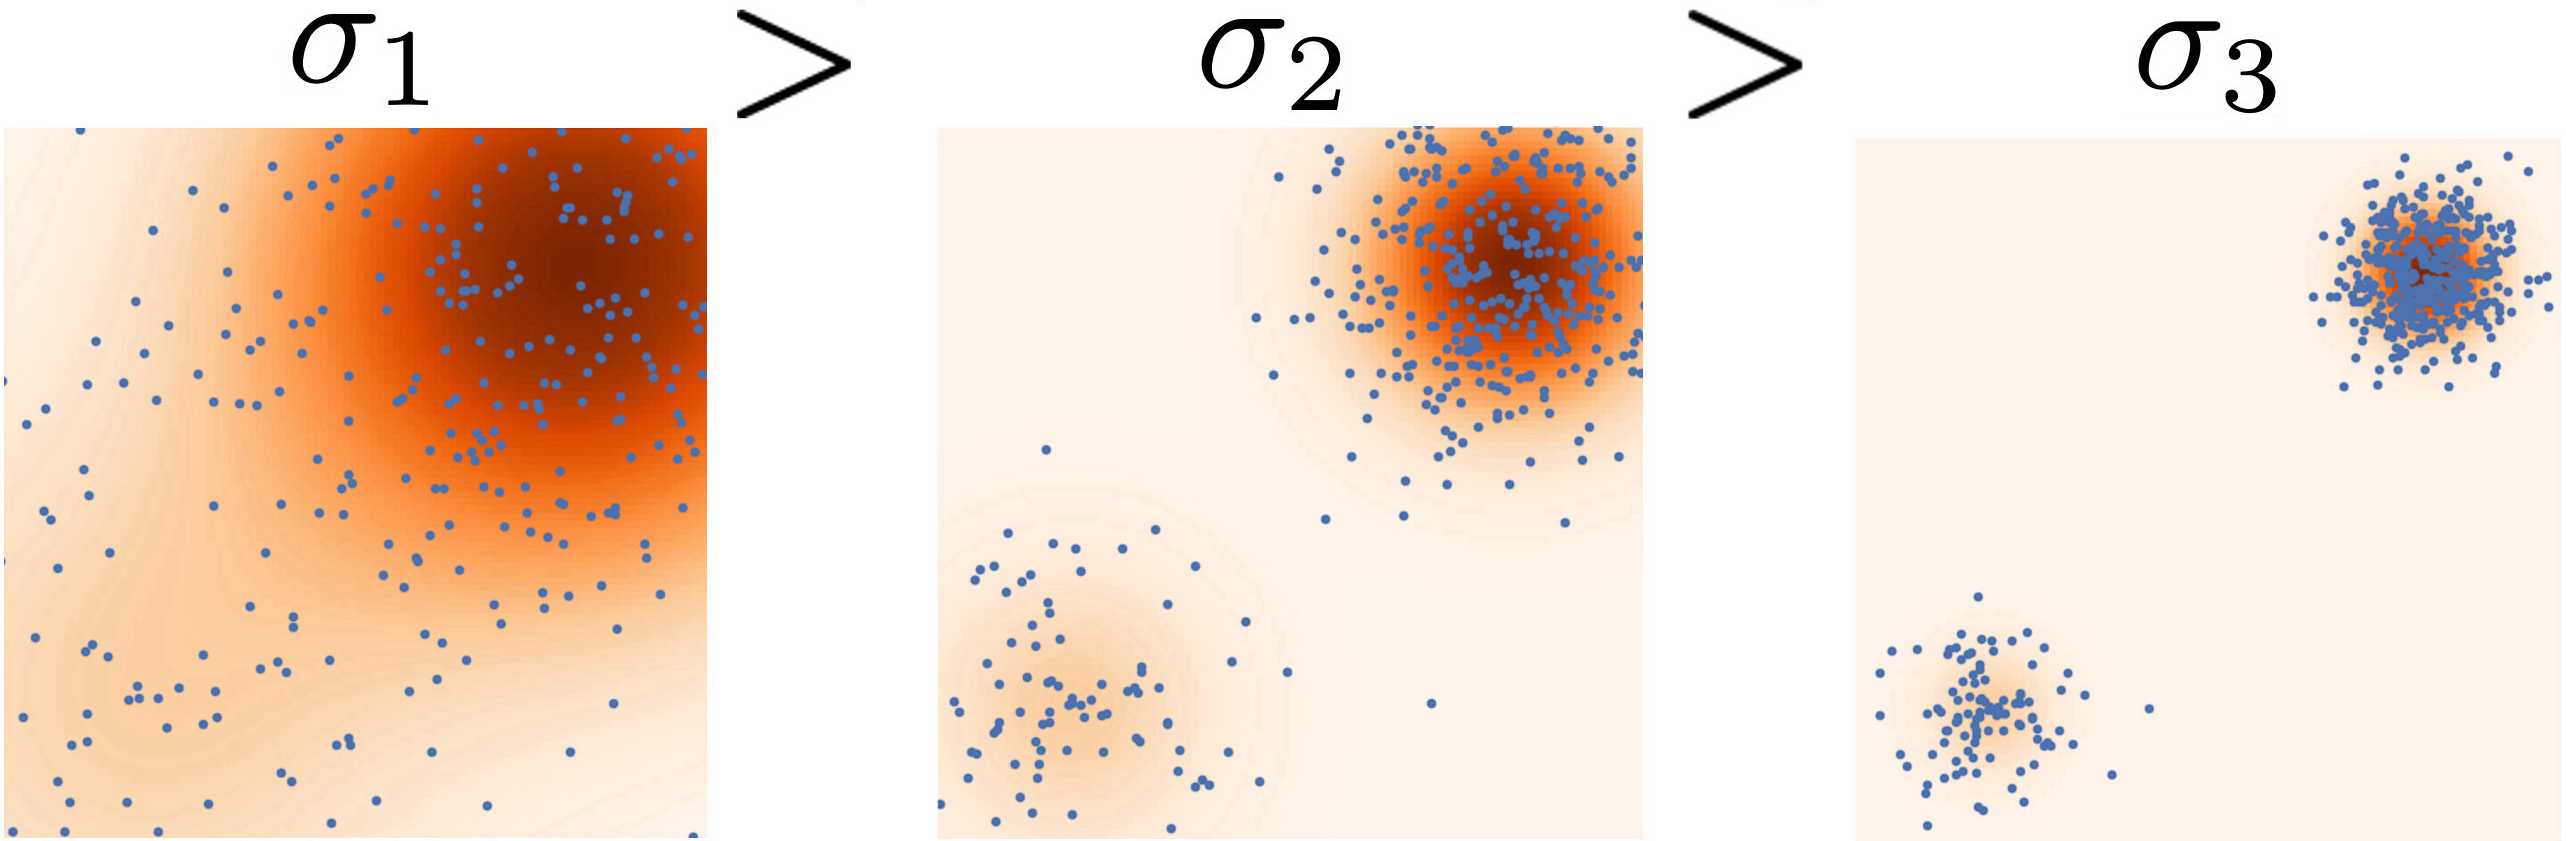
\includegraphics[width=0.6\linewidth]{figs/multi_scale}
	\end{figure}
	\begin{figure}
		
\includegraphics[width=\linewidth]{figs/duoduo}
	\end{figure}
	\myfootnotewithlink{https://arxiv.org/abs/1907.05600}{Song Y. et al. Generative Modeling by Estimating Gradients of the Data Distribution, 2019}
\end{frame}
%=======
\begin{frame}{Noise conditioned score network}
	
	\begin{minipage}{0.5\linewidth}
		\vspace{-0.7cm}
		\begin{block}{Training: loss function}
			\vspace{-0.8cm}
			\[
			\sum_{i=1}^L \sigma_l^2\bbE_{\pi(\bx')} \bbE_{\bepsilon}\left\| \bs_l + \frac{\bepsilon}{\sigma_l} \right\|^2_2,
			\]
		\end{block}
		\vspace{-0.5cm}
		Here
		\begin{itemize}
			\item $\bs_l = \bs(\bx' + \sigma_l \cdot \bepsilon, \btheta, \sigma_l)$.
			\item $\nabla_{\bx} \log p(\bx | \bx', \sigma) = - \frac{\bx - \bx'}{\sigma^2} = - \frac{\bepsilon}{\sigma_l}$.
		\end{itemize}
	\end{minipage}%
	\begin{minipage}{0.5\linewidth}
		\begin{block}{Inference: annealed Langevin dynamic}
			\begin{figure}
				\includegraphics[width=0.9\linewidth]{figs/ald}
			\end{figure}
		\end{block}
	\end{minipage}
	\vspace{-0.7cm}
	\begin{block}{Samples}
		\begin{figure}
			\includegraphics[width=\linewidth]{figs/NCSNv2}
		\end{figure}
	\end{block}
	\myfootnotewithlink{https://arxiv.org/abs/2006.09011}{Song Y. et al. Improved Techniques for Training Score-Based Generative Models, 2020}
\end{frame}
%=======
\section{Gaussian diffusion process}
%=======
\begin{frame}{Forward gaussian diffusion process}
	Let $\bx_0 = \bx \sim \pi(\bx)$, $\beta \in (0, 1)$. Define the Markov chain
	\[
		\bx_t = \sqrt{1 - \beta} \cdot \bx_{t - 1} + \sqrt{\beta} \cdot \bepsilon, \quad \text{where }\bepsilon \sim \cN(0, 1);
	\]
	\[
		q(\bx_t | \bx_{t-1}) = \cN(\bx_t | \sqrt{1 - \beta} \cdot \bx_{t-1}, \beta \cdot \bI).
	\]
	\vspace{-0.6cm}
	\begin{block}{Statement 1}
		Applying the Markov chain to samples from any $\pi(\bx)$ we will get $\bx_{\infty} \sim p_{\infty}(\bx) = \cN(0, 1)$. Here $p_{\infty}(\bx)$ is a \textbf{stationary} distribution:
		\vspace{-0.2cm}
		\[
			p_{\infty}(\bx) = \int q(\bx | \bx') p_{\infty}(\bx') d \bx'. 
		\]
		\vspace{-0.8cm}
	\end{block}
	\begin{block}{Statement 2}
		Denote $\bar{\alpha}_t = \prod_{s=1}^t (1 - \beta_s)$. Then 
		\vspace{-0.2cm}
		\[
			\bx_t = \sqrt{\bar{\alpha}_t} \cdot \bx_{0} + \sqrt{1 - \bar{\alpha}_t} \cdot \bepsilon, \quad \text{where } \bepsilon \sim \cN(0, 1)
		\]
		\vspace{-0.7cm}
		\[
			q(\bx_t | \bx_0) = \cN(\bx_t | \sqrt{\bar{\alpha}_t} \cdot \bx_0, (1 - \bar{\alpha}_t) \cdot \bI).
		\]
		We could sample from any timestamp using only $\bx_0$!
	\end{block}
	\myfootnotewithlink{http://proceedings.mlr.press/v37/sohl-dickstein15.pdf}{Sohl-Dickstein J. Deep Unsupervised Learning using Nonequilibrium Thermodynamics, 2015}
\end{frame}
%=======
\begin{frame}{Forward gaussian diffusion process}
	\textbf{Diffusion} refers to the flow of particles from high-density regions towards low-density regions.
	\vspace{-0.2cm}
	\begin{figure}
		\includegraphics[width=0.5\linewidth]{figs/diffusion_over_time}
	\end{figure}
	\vspace{-0.6cm}
	\begin{enumerate}
		\item $\bx_0 = \bx \sim \pi(\bx)$;
		\item $\bx_t = \sqrt{1 - \beta} \cdot \bx_{t - 1} + \sqrt{\beta} \cdot \bepsilon$, where $\bepsilon \sim \cN(0, 1)$, $t \geq 1$;
		\item $\bx_T \sim p_{\infty}(\bx) = \cN(0, 1)$, where $T >> 1$.
	\end{enumerate}
	If we are able to invert this process, we will get the way to sample $\bx \sim \pi(\bx)$ using noise samples $p_{\infty}(\bx) = \cN(0, 1)$. \\ 
	Now our goal is to revert this process.
	\myfootnotewithlink{https://ayandas.me/blog-tut/2021/12/04/diffusion-prob-models.html}{Das A. An introduction to Diffusion Probabilistic Models, blog post, 2021}
\end{frame}
%=======
\begin{frame}{Reverse gaussian diffusion process}
	\vspace{-0.3cm} 
	\begin{figure}
		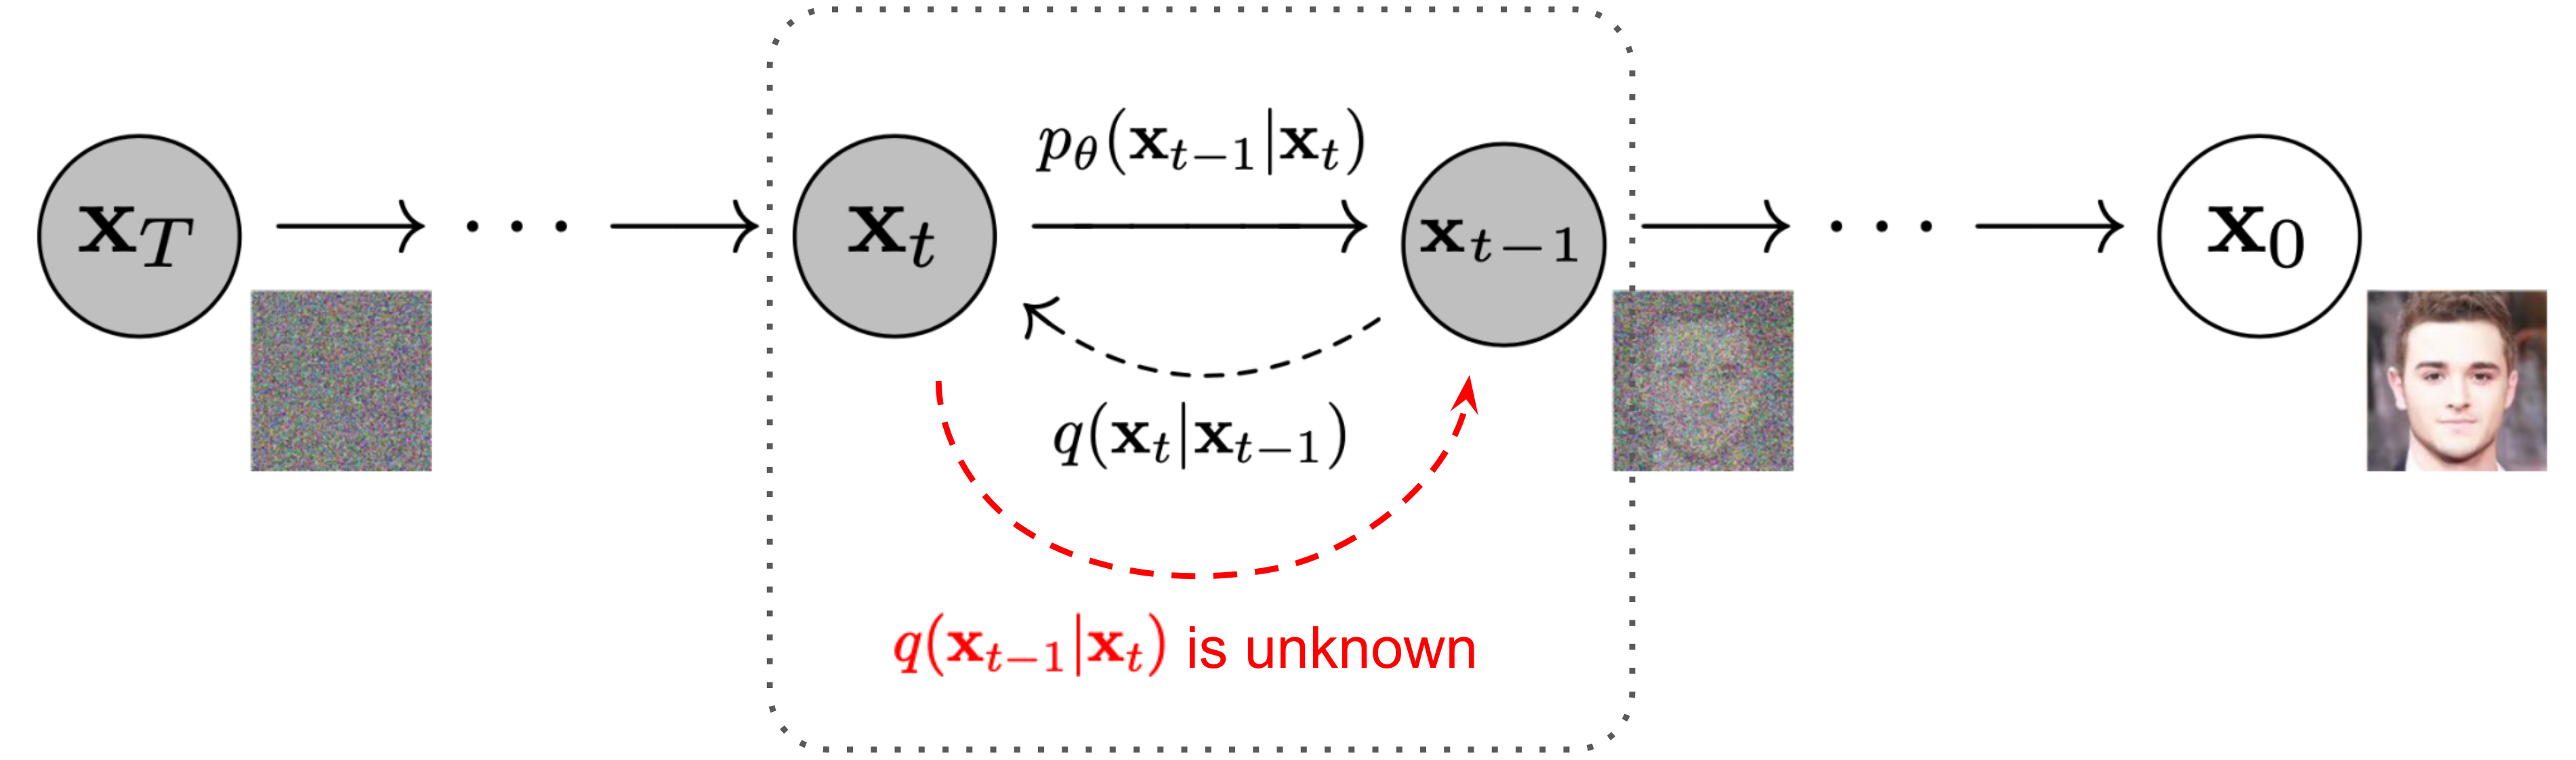
\includegraphics[width=0.8\linewidth]{figs/DDPM}
	\end{figure}
	\vspace{-0.3cm} 
	Let define the reverse process
	\vspace{-0.2cm}
	\[
		p(\bx_{t - 1} | \bx_t, \btheta) = \cN \bigl(\bx_{t - 1} | \bmu(\bx_t, \btheta, t), \bsigma^2(\bx_t, \btheta, t)\bigr)
	\]
	\vspace{-0.5cm}
	\begin{minipage}{0.5\linewidth}
		\begin{block}{Forward process}
			\begin{enumerate}
				\item $\bx_0 = \bx \sim \pi(\bx)$;
				\item $\bx_t = \sqrt{1 - \beta} \cdot \bx_{t - 1} + \sqrt{\beta} \cdot \bepsilon$, where $\bepsilon \sim \cN(0, 1)$, $t \geq 1$;
				\item $\bx_T \sim p_{\infty}(\bx) = \cN(0, 1)$.
			\end{enumerate}
		\end{block}
	\end{minipage}%
	\begin{minipage}{0.5\linewidth}
		\begin{block}{Reverse process}
			\begin{enumerate}
				\item $\bx_T \sim p_{\infty}(\bx) = \cN(0, 1)$;
				\item $\bx_{t - 1} = \bsigma(\bx_t, \btheta, t) \cdot \bepsilon + \bmu(\bx_t, \btheta, t)$;
				\item $\bx_0 = \bx \sim \pi(\bx)$;
			\end{enumerate}
		\end{block}
	\end{minipage}
	\textbf{Note:} The forward process does not have any learnable parameters!
	\myfootnotewithlink{https://lilianweng.github.io/posts/2021-07-11-diffusion-models/}{Weng L. What are Diffusion Models?, blog post, 2021}
\end{frame}
%=======
\begin{frame}{Summary}
	\begin{itemize}
		\item Score matching proposes to minimize Fisher divergence to get score function.
		\vfill
		\item Sliced score matching and denoising score matching are two techniques to get scalable algorithm for fitting Fisher divergence.
		\vfill
		\item Noise conditioned score network uses multiple noise levels and annealed Langevin dynamics to fit score function.
		\vfill
		\item Gaussian diffusion process is a Markov chain that injects special form of Gaussian noise to the samples.
		\vfill
		\item Reverse process allows to sample from the real distribution $\pi(\bx)$ using samples from noise.
	\end{itemize}
\end{frame}
\end{document} 